\chapter{Modelización}
\label{ch:modelizacion}
\lhead{\emph{Modelización}}

\section{Modelo de la antena}

El modelo de antena está programado de tal forma que se lo pueda utilizar para simular una antena con parámetros de RF,
la misma está conformada por los siguientes componentes: cables, psc, trms, desfasadores y elementos radiantes. 

La modelizaci\'on de los componentes en RF se realiza utilizando los par\'ametros S. En el apéndice \ref{AppendixC} se muestra 
un ejemplo de estos archivos para una antena de dos elementos radiantes.

Como es necesario realizar ensayos de montecarlo utilizando distintos tipos de calibraciones ante una misma configuración y 
comportamiento de antena, se optó por guardar en disco dicha información utilizando archivos json. En los cuales se guarda la
configuración y propiedades físicas tanto del panel como de la RFDN. Las propiedades del primer grupo son, simplemente, las 
distancias entre todos los elementos. Las del segundo grupo corresponden a la matriz de parámetros S y la interconexión entre 
componentes. En el anexo \ref{AppendixC} se puede observar un ejemplo de estos archivos para una antena con dos elementos 
radiantes.

Dado lo mencionado previamente, el simulador consta de dos etapas, la primera parte es la encargada de la modelización
de la antena y sus componentes; y la segunda, de calibrar dicho modelo. La figura \ref{fig:prog_inic} muestra de forma 
simplificada el flujo de ejecuci\'on del programa.

\begin{figure}
 \centering
 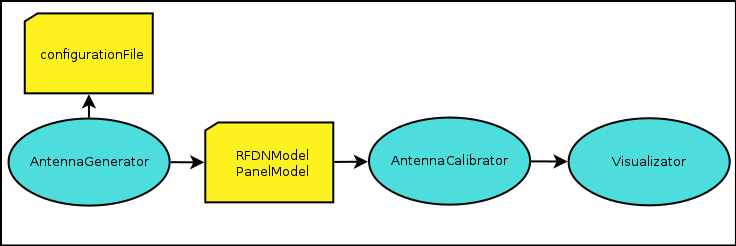
\includegraphics[width=10cm]{gfx/FlujoEjecucion.png}
 \caption{Flujo de ejecuci\'on del modelo de antena.}
 \label{fig:prog_inic}
\end{figure}


\subsection{Generador de Antena}

En principio, una antena necesita que todos los caminos entre el punto donde se inyecta o recibe la se\~nal y los m\'odulos 
radiantes sean iguales. Esta caracter\'istica es similar a la de un \'arbol balanceado. Por lo tanto, para definir la 
estructura interna de la antena, se definen simplemente los elementos que conforman dicho \'arbol y, para determinar el orden 
de armado de la antena, se utiliza una lista. El orden es descendiente, si se para en un elemento de la lista, los de la 
izquierda son ascendientes y los de la derecha son descendientes. En la figura \ref{fig:2RMAntenna} se muestra la antena que 
se construye teniendo como configuración: [\enquote*{cable1}, \enquote*{psc12}, \enquote*{cable2}, \enquote*{trm}, 
\enquote*{circulator}, \enquote*{cable3}, \enquote*{rm}].

\begin{figure}
 \centering
 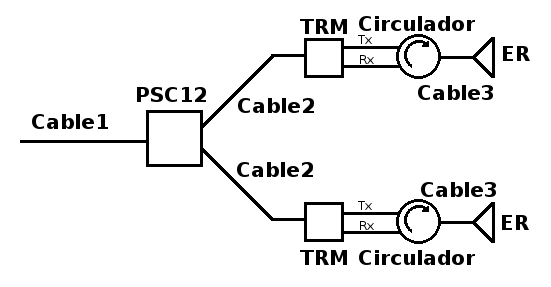
\includegraphics[width=10cm]{gfx/RFDN.png}
 \caption{Estructura interna de una de las polarizaciones de una antena con dos elementos radiantes.}
 \label{fig:2RMAntenna}
\end{figure}

Es necesario definir las características físicas de cada uno de los elementos que componen la antena. La tabla 
\ref{tab:propertiesOfComponents} determina las propiedades de cada uno.

\begin{table}[H]
  \footnotesize
  \centering
  \begin{tabular}{|c|c|}
	\hline
	\textbf{Componente de Antena} & \textbf{Cacarcterísticas físicas} \tabularnewline \hline 
	\multirow{2}{*}{cable} &  attenuation [db] \tabularnewline \cline{2-2}
	 & length [m] \tabularnewline \hline 
	\multirow{3}{*}{TRM} & isDead \tabularnewline \cline{2-2}
	 & gain [db]\tabularnewline \cline{2-2}
	 & phaseShift [deg] \tabularnewline \hline 
	PSC1$j$ & outputPorts = $j$ \tabularnewline \hline 
	circulator & \tabularnewline \hline 
	RM & \tabularnewline \hline 
  \end{tabular}
  \caption{Propiedades físicas de cada componente de una antena}
  \label{tab:propertiesOfComponents}
\end{table}

Como es necesario que la representación de las propiedades mencionadas previamente sean representativas en radio frecuencia,
se utilizan los parámetros S (como se menciona en el capítulo \ref{ch:phasedArray}). En la figura \ref{fig:creationPackage} 
se muestra el diagrama de clases donde se puede observar que el creador de antena hace uso de los generadores de parámetros S 
de cada componente.

\begin{figure}
 \centering
 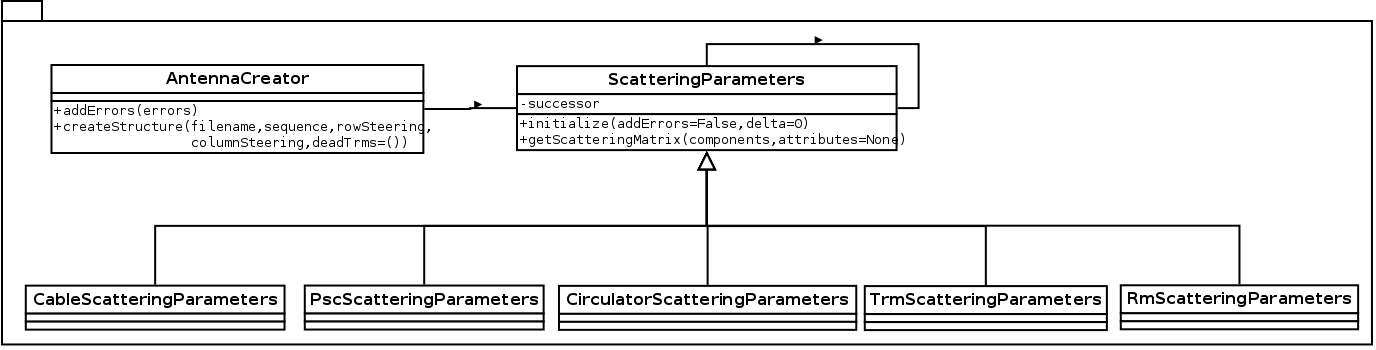
\includegraphics[width=15cm]{gfx/creationPackage.png}
 \caption{Diagrama de clases del generador de antena.}
 \label{fig:creationPackage}
\end{figure}

Con la RFDN, si bien está definida la cantidad de elementos radiantes, falta definir las dimensiones de la antena, 
en otras palabras, la cantidad de paneles, la cantidad de elementos por panel y la separación, tanto horizontal como vertical,
entre elementos. Los primeros se traducen a cantidad de columnas y filas de RMs. 

Como dicha información es redundante y posiblemente incompatible con la definición de la estructura interna de la antena, es 
necesario un chequeo de compatibilidad. La figura \ref{fig:frontAntenna} muestra el frente de una antena que se construye 
teniendo como configuración: "quantityRows": 1, "quantityColumns": 2, "verticalSeparation": 0.2 y "horizontalSeparation": 0.2.

\begin{figure}
 \centering
 
\includegraphics[width=4cm]{gfx/FrontAntenna2.png}
 \caption{Frente de antena de dos elementos radiantes.}
 \label{fig:frontAntenna}
\end{figure}

Una vez obtenida la estructura de la antena, es necesario determinar que componentes van a tener desvíos en el comportamiento 
deseado. Para ello, se agrega una lista indicando los componentes con errores. Las incertidumbres tienen una distribución 
gaussiana con media 0. El desvío estándar es configurable.

Si se deseara realizar la calibración en modo completo, se deberían agregar errores de planitud de la antena. Con lo cual, 
dichos desvíos se verían reflejados en el archivo de la configuración del panel de la antena. En la presente tesis solamente 
se desarrolló el modelo con planitud ideal.

\subsection{Calibrador}

En la figura \ref{fig:modelPackage} se muestra el diagrama de clases del calibrador del modelo de antena. Se puede observar que
la clase Antena, la cual pertenece al modelo, modeliza el comportamiento de todos sus componentes. Los calibradores pueden ser 
el clásico o el de acoplamientos mutuos; el primero utiliza un creador de señales chirp y de códigos walsh, en cambio, el 
segundo utiliza clases del tipo MatrixCalibratorBuilder, las cuales tienen distintas estrategias para generar ecuaciones en base
a los lazos de calibración generados.

\begin{figure}
 \centering
 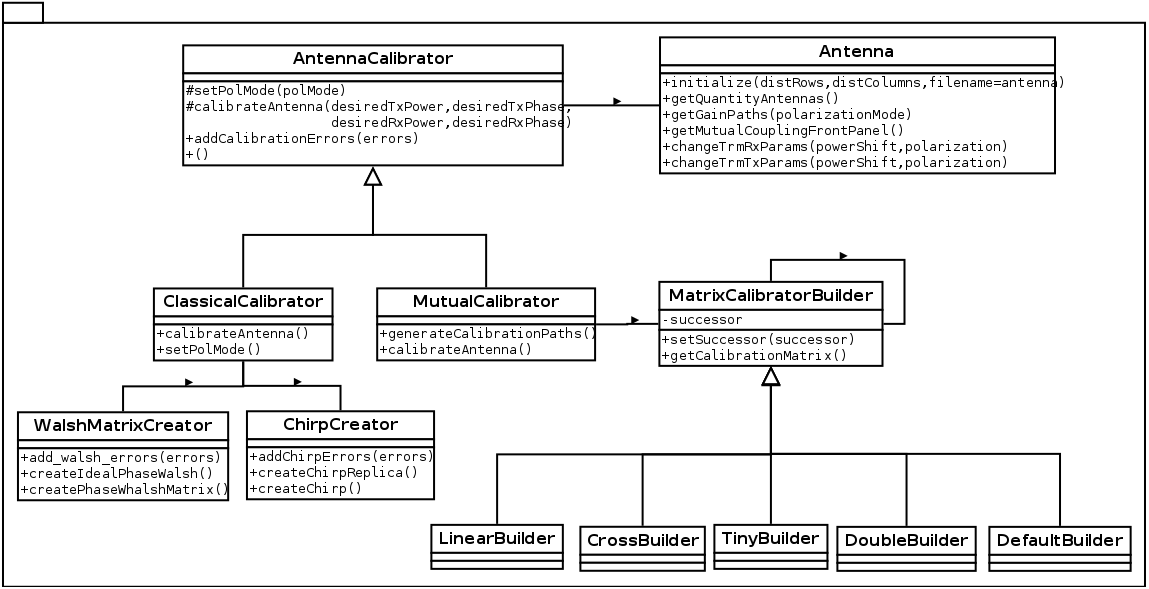
\includegraphics[width=15cm]{gfx/modelPackage.png}
 \caption{Diagrama de clases del calibrador de antena.}
 \label{fig:modelPackage}
\end{figure}


A la hora de calibrar, los primeros parámetros a definir son la potencia (en dB), fase (en grados) y frecuencia (en Hz) de la 
señal utilizada con que se alimenta la antena para ser transmitida. A su vez, se debe definir el apuntamiento deseado. Para 
ello, se tienen que configurar la fase de los desfasadores en transmisión de la polarización a transmitir, tomando en cuenta lo 
explicado en la sección \ref{ssec:beamSteering}. Estos valores están definidos en el archivo de configuración bajo el nombre 
de \enquote*{Row Steering} y \enquote*{Column Steering}. Los mismos se traducen como el apuntamiento vertical y horizontal 
respectivamente de la antena.

Una vez definidos los parámetros previamente mencionados, se puede obtener la ganancia de la antena en las partes de 
transmisión y recepción para crear los lazos de calibración. Dichas ganancias están definidas como matrices de parámetros
S y se las obtiene realizando los siguientes pasos.

\begin{enumerate}
	\item Se recorre recursivamente la estructura de la antena, se van leyendo los parámetros S de cada componente y se va 
		armando una lista de caminos distintos.
	\item Si el componente tiene más de un puerto de salida, se agranda la lista de elementos encontrados. La lista final tiene 
		tantos elementos como RMs tiene la antena.
	\item A la matriz leída se la transforma en parámetros T utilizando la transformación definida en la sección 
		\ref{ssec:conversion} y se la multiplica con los datos guardados en la lista de elementos encontrados. Se realiza esto 
		por la propiedad de multiplicación entre matrices de transferencia definida en la sección \ref{ssec:transMatrix}.
	\item Una vez recorrida toda la antena, la lista de parámetros T se la convierte nuevamente a parámetros S.
	\item Si los parámetros S son para recepción de la antena, se deben intercambiar los elementos de la matriz. $S_{11}$ con 
		$S_{22}$ y $S_{21}$ con $S_{12}$.
\end{enumerate}

Para armar los lazos de calibración, se tiene que tener en cuenta distintos tipos de errores que pueden afectar a los mismos, 
los cuales son: error de ganancia entre pulsos, error de ganancia de la chirp replica y error de fase del walsh. Todos estos 
errores son tratados como gaussianos con media igual a cero.

Desvíos de ganancia o fase entre pulsos: Esta incertidumbre se puede dar por inestabilidades en el oscilador local que genera 
la señal a transmitir/calibrar la antena o incertidumbres de medición del receptor.

Desvíos de ganancia o fase de la chirp replica: Esta incertidumbre se da por el cambio de comportamiento del lazo de 
calibración donde se mide la chirp réplica, como dicho lazo está caracterizado, cuando cambia su valor de ganancia, esta 
variación es atribuida a la chirp en vez de al lazo.

Desvíos de fase del walsh: Esta incertidumbre aparece a causa de las diferencias de comportamiento real y configurado en los 
desfasadores. 

Los lazos de calibración dependen del método utilizado, los cuales se explicarán a continuación.

\subsubsection{Calibración clásica}
Para armar los datos a ser calibrados, todos los lazos (que abarcan hasta los módulos TR de la RFDN) se los multiplica con 
tantas chirps como el método indica, con los errores que deba tener (según configuración) y con la codificación del código 
walsh siguiendo lo especificado en la sección \ref{ssc:classicalMethod}. El resultado es una matriz adquirida, la cual, para
decodificar y obtener la ganancia/fase de un TRM, se lo debe multiplicar por un conjunto de chirp réplicas desfasadas según la 
columna del código Walsh al que perteneciente el TRM. 

\subsubsection{Calibración con acoplamientos mutuos}

Para obtener los distintos lazos de calibración se desarrollaron varias estrategias a saber: 

\begin{itemize}
	\item \textbf{LinearBuilder:} Esta estrategia construye ecuaciones utilizando la resta de dos lazos que tengan un elemento en 
		común, llamado central. Dicho elemento puede ser utilizado para transmitir o recibir, dependiendo si se desea obtener una 
        ecuación de Rx o Tx respectivamente. El método requiere que las distancias del elemento en común al resto sean iguales
		para poder eliminar los acoplamientos mutuos y que los tres componentes estén alineados entre sí.
         
		Para ejemplificar, en la figura \ref{fig:linealBuilder} se pueden observar dos pares de lazos de calibración. Si se resta el
        azul con el verde, aprovechando que $C_{14} = C_{74}$, se obtiene una ecuación de la rama de transmisión; en cambio, 
        si se resta el rojo con el amarillo, aprovechando que $C_{53} = C_{57}$, se obtiene una ecuación de la rama de 
        recepción de la antena.
			
		\begin{figure}[H]
		 \centering
		 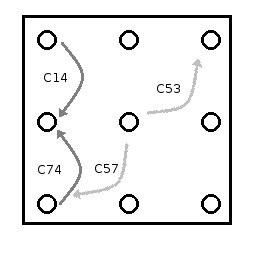
\includegraphics[width=5cm]{gfx/linearBuilder.png}
		 \caption{Estrategia LinearBuilder. Restar azul con verde para transmisión y restar rojo con amarillo para recepción.}
		 \label{fig:linealBuilder}
		\end{figure}

	\item \textbf{CrossBuilder:} Esta estrategia construye ecuaciones utilizando la resta de dos lazos que tengan un elemento en 
		común, llamado central. Dicho elemento puede ser utilizado para transmitir o recibir como en el LinearBuilder. La única 
        diferencia es que en vez de requerir que los tres elementos estén alineados, tienen que formar una L. En otras palabras,
        las rectas de unión deben ser perpendiculares entre sí.
		
        Para ejemplificar, en la figura \ref{fig:crossBuilder} se pueden observar dos pares de lazos de calibración. Si se resta el
        azul con el verde, aprovechando que $C_{12} = C_{14}$, se obtiene una ecuación de la rama de recepción. En cambio, 
        si se resta el rojo con el amarillo, aprovechando que $C_{53} = C_{59}$, se obtiene una ecuación de la rama de 
        transmisión de la antena.

		\begin{figure}[H]
		 \centering
		 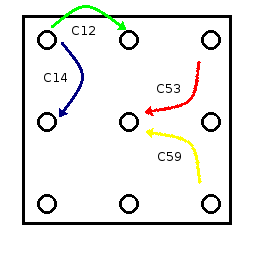
\includegraphics[width=5cm]{gfx/crossBuilder.png}
		 \caption{Estrategia CrossBuilder.}
		 \label{fig:crossBuilder}
		\end{figure}

	\item \textbf{TinyBuilder:} Esta estrategia construye ecuaciones solamente si la cantidad de elementos en alguna dirección, 
        horizontal o vertical, es igual a dos. Utilizando los cuatro lazos de calibración posibles por cada par de elementos 
		que hay en la dirección previamente mencionada, resta los lazos transmitidos por un elemento con los del otro. El resultado 
		es la resta de las dos ramas de transmisión. Para obtener ecuaciones de la diferencia en recepción el razonamiento es 
		análogo, se deben restar los lazos recibidos de uno con los del otro elemento.

        Para ejemplificar, la figura \ref{fig:tinyBuilder} muestra una antena de dos elementos en configuración vertical. En 
        esta estrategia se restan los caminos azules con los verdes aprovechando que $C_{11} = C_{22}$ y que $C_{12} = C_{21}$.
		
		\begin{figure}[H]
		 \centering
		 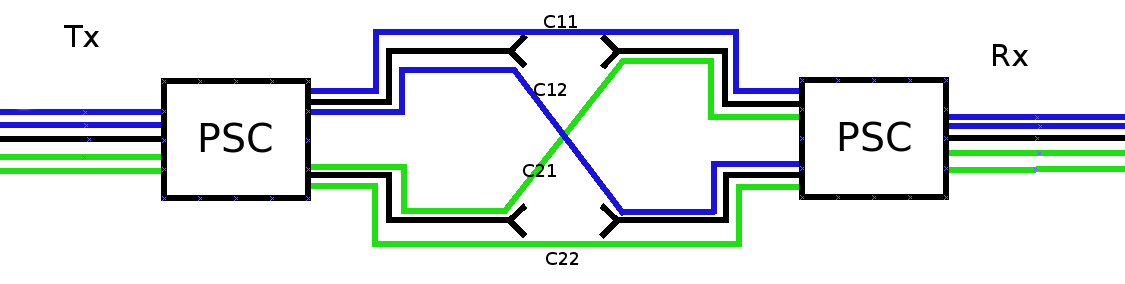
\includegraphics[width=10cm]{gfx/tinyBuilder.png}
		 \caption{Estrategia TinyBuilder.}
		 \label{fig:tinyBuilder}
		\end{figure}

        Nota: En la figura \ref{fig:tinyBuilder} se puede llegar a la interpretación que hay 4 elementos radiantes en vez 
        de 2. Cada elemento fue duplicado para enfatizar que la polarización de transmisión es diferente a la de recepción.

	\item \textbf{DoubleBuilder:} Esta estrategia construye ecuaciones solamente si la cantidad de elementos radiantes de la 
        antena, en cualquiera de sus direcciones, es distinta de dos. A diferencia de la estrategia TinyBuilder, también se 
        utilizan las ramas de recepción de elementos que tengan las mismas distancias a los elementos transmisores.
        
        Para ejemplificar, se tiene una antena de 5 elementos en configuración vertical, como se muestra en la figura 
		\ref{fig:doubleBuilder}. Esta estrategia resta los caminos azules con los verdes aprovechando que $C_{12} = C_{54}$ y que
		$C_{14} = C_{52}$ (por simetría de la antena), dando como resultado dos veces la resta de las ramas de transmisión.
		
		\begin{figure}[H]
		 \centering
		 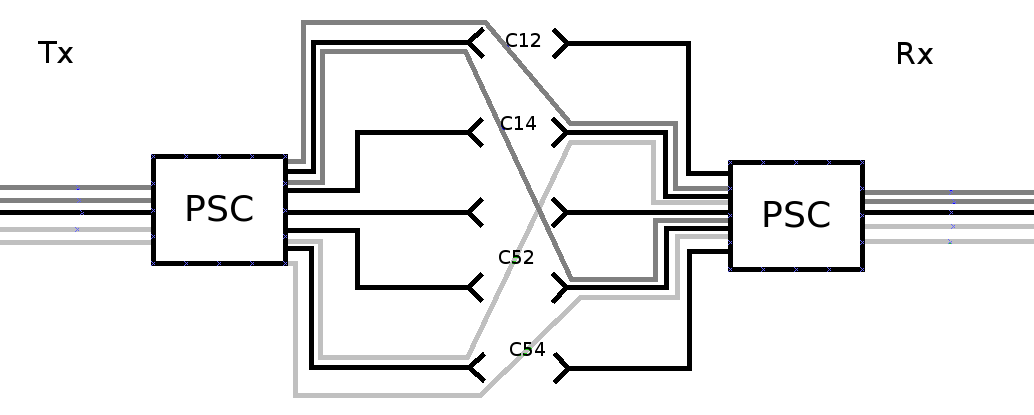
\includegraphics[width=10cm]{gfx/doubleBuilder.png}
		 \caption{Estrategia DoubleBuilder. Al restar los lazos azules con los verdes queda solo la resta de la cadena en 
         transmisión.}
		 \label{fig:doubleBuilder}
		\end{figure}

        Nota: En la figura \ref{fig:doubleBuilder} se puede llegar a la interpretación que hay 10 módulos radiantes en vez 
        de 5. Cada elemento fue duplicado para enfatizar que la polarización de transmisión es diferente a la de recepción.

	\item \textbf{DefaultBuilder:} Esta estrategia se la utiliza para agregar las ecuaciones donde se mide la potencia 
		transmitida/recibida para que el resultado del método sea único. Por ejemplo, puede ser el resultado de la medición de un 
		TRM obtenido de la calibración clásica.
\end{itemize}


Una vez obtenidas todas las ecuaciones de las calibraciones, se procede a utilizar el método de cuadrados mínimos definido en 
la sección \ref{sec:meanSquare}. Para la fase, hay que tener extremo cuidado por su naturaleza modular, por lo tanto, 
previamente a la realización del cálculo de cuadrados mínimos, se acomoda el conjunto de resultados de acuerdo a la sección 
\ref{ssc:mutualPhase}.

\subsection{Configuraciones del sistema}

A modo de resumen, se lista en la tabla \ref{tab:conf_modelo_antena} todas las posibles configuraciones en el modelo para 
realizar los distintos ensayos.

\begin{center}
  \footnotesize
  \centering
  \begin{longtable}{|c|p{9cm}|}
    \hline 
	\multicolumn{2}{|c|}{\textbf{Parámetros de entrada}} \\ 
	\hline
    Frequencia		& Es la frecuencia central de trabajo en Hz \tabularnewline \hline 
    Potencia		& Potencia con la que se alimenta la antena en db \tabularnewline \hline 
    Fase			& Fase con la que se alimenta la antena en grados \tabularnewline \hline 
    Row Steering	& Apuntamiento horizontal que se le quiere dar a la señal transmitida, en grados  \tabularnewline \hline 
    Column Steering	& Apuntamiento vertical que se le quiere dar a la señal transmitida, en grados  \tabularnewline \hline 
	\multicolumn{2}{|c|}{\textbf{Parámetros de calibración}} \\ 
	\hline
	potencia Tx deseada	& Potencia de transmisión deseada para calibrar  \tabularnewline \hline 
	potencia Rx deseada	& Potencia de recepción deseada para calibrar  \tabularnewline \hline 
	Errores	& Son los errores referentes a la hora de calibrar el modelo de antena. Pueden ser: interPulseGainChirpError, 
	interPulsePhaseChirpError, gainChirpRepError, phaseChirpRepError, WalPhaseErrors  \tabularnewline \hline
	\multicolumn{2}{|c|}{\textbf{Parámetros de Antena}} \\ 
	\hline
	Cantidad Filas	& Da la cantidad de módulos radiantes en dirección vertical \tabularnewline \hline 
	Cantidad Columnas	& Da la cantidad de módulos radiantes en dirección horizontal \tabularnewline \hline 
	Separación vertical & Es la separación vertical entre RMs \tabularnewline \hline 
	Separación horizontal & Es la separación horizontal entre RMs \tabularnewline \hline 
	Secuencia de componentes & Es la secuencia de componentes que conforma la RFDN, los mismos pueden ser: cables, psc, trm, circulador, rm \tabularnewline \hline 
	Errores  & Son los componentes de la antena que pueden tener errores. Los mismos pueden ser: RMError, TRMError, CirculatorError, PSCError \tabularnewline \hline 
	TRMs muertos & Es una lista que indica que trms están muertos en el panel de la antena. \tabularnewline \hline 
	\multicolumn{2}{|c|}{\textbf{Componentes de Antena}} \\
	\hline
	$cable_i$ & Se pueden definir tantos cables como se deseen, los parámetros a definir son: attenuation [db], length [m], type = cable \tabularnewline \hline 
	$trm_i$ & Se pueden definir tantos TRMs como se deseen, los parámetros a definir son: gain [db], phaseShift [deg], type = TRM \tabularnewline \hline 
	$psc_{1j}$ & Se pueden definir tantos PSC como se deseen, los parámetros a definir son: outputPorts = $j$, type = PSC1$j$ \tabularnewline \hline 
	circulator & aca se puede definir un circulador, el parámetro a definir es: type = circulator \tabularnewline \hline 
	$rm$ & Se puede definir un RM, el parámetro a definir es: type = RM \tabularnewline \hline 
	\multicolumn{2}{|c|}{\textbf{Desvío estándar del error}} \\
	\hline
	Error del cable & Desvío estándar de los cables. \tabularnewline \hline 
	Error del circulador & Desvío estándar de los circuladores. \tabularnewline \hline 
	Error del TRM & Desvío estándar de los TRMs. \tabularnewline \hline 
	Error del PSC & Desvío estándar de los PSC. \tabularnewline \hline 
	Error del RM & Desvío estándar de los RM. \tabularnewline \hline 
	Error de ganancia entre pulsos & Desvío estándar de ganancia entre pulsos de calibración. \tabularnewline \hline 
	Error de fase entre pulsos & Desvío estándar de fase entre pulsos de calibración. \tabularnewline \hline 
	Error de ganancia de la chirp replica & Desvío estándar de ganancia de la chirp replica. \tabularnewline \hline 
	Error de fase de la chirp replica & Desvío estándar de fase de la chirp replica. \tabularnewline \hline 
	Error de fase del walsh & Desvío estándar de fase de la configuración de los desfasadores en calibración. \tabularnewline \hline 
	\caption{Configuraciones del modelo de antena}
  \end{longtable}
  \label{tab:conf_modelo_antena}
\end{center}

A su vez, también se puede configurar que tipo de calibración se desea correr para poder obtener los resultados y se pueden 
graficar tanto los diagramas de radiación obtenidos en algún corte en azimuth/rango o el conjunto de ganancias y fases con 
respecto al valor ideal. La figura \ref{fig:visualPackage} muestra el diagrama de clases del visualizador.

\begin{figure}[H]
 \centering
 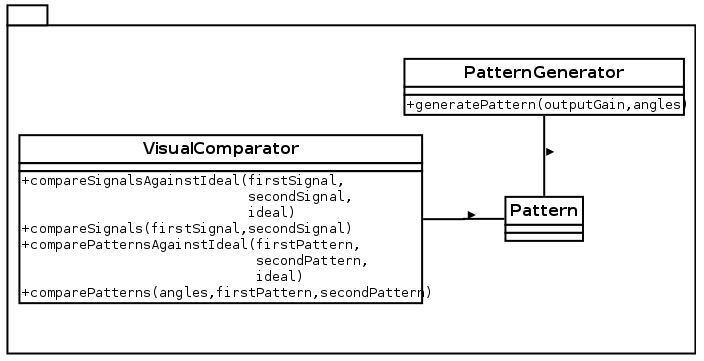
\includegraphics[width=11cm]{gfx/visualPackage.png}
 \caption{Diagrama de clases de los visualizadores.}
 \label{fig:visualPackage}
\end{figure}

